% !TEX TS-program = XeLaTeX
% The next lines tell TeXShop to typeset with xelatex, and to open and save the source with Unicode encoding.

%!TEX encoding = UTF-8 Unicode
% !BIB TS-program =

\documentclass[12pt]{article}

\usepackage{uproposal2}
\usepackage{textcomp}

%\usepackage{draftwatermark}
%\SetWatermarkText{DRAFT}
%\SetWatermarkScale{1}

\title{Preliminary Proposal to Encode Californian\\\normalsize \sf (Individual Submission)}
\author{Steven R.~Loomis — srl295@gmail.com\\\small\url{https://srl295.github.io}}

\date{2020-04-01}


\makeindex

\begin{document}

\newfontfamily\calfont{Californian}
\newcommand\Cal[1]{{\calfont #1}}
% \newcommand{\Cal}[1]{\fontspec{Californian}#1\fontspec{Computer Modern}}


\maketitle

\section{Introduction}
% \addcontentsline{toc}{section}{Introduction}

This is a proposal to encode the characters of a new script, Californian.

\section{Background}

Californian is a language spoken by lots of people on the western coast of the USA.
The two dialects, Northern and Southern, are mutually unintelligable due to differences
in vocabulary and word order. Both dialects, however, are written using the same script.

\section{Orthography}

Californian is written from left to right, with flowing lines from top to bottom.
Research is ongoing, but at this time six letters are attested, and they are being
proposed for encoding.

\section{Repertoire}

The proposed repertoire consists of exactly 6 characters, plus one combining sign.
Other Punctuation will
be drawn from the usual characters.

\subsection{Base Letters}

The three base letters are given below.

\begin{table}[h]
    \centering
    \caption{Base Letters}
    \begin{tabular}{| l | l | c |}
        \hline
            Character & Codepoint & Glyph \\
        \hline
        {\tt CALIFORNIAN LETTER F} & \tt{U+F046} & \Cal{F} \\
        {\tt CALIFORNIAN LETTER R} & \tt{U+F052} & \Cal{R} \\
        {\tt CALIFORNIAN LETTER I} & \tt{U+F049} & \Cal{I} \\
        \hline
        \hline
    \end{tabular}
\end{table}


\subsection{Combining Signs}

The combining Kumquat  \Cal{~\_} is used to form three additional letters, \Cal{F\_} ~, \Cal{R\_} ~and \Cal{I\_}

\begin{table}[h]
    \centering
    \caption{Combining Signs}
    \begin{tabular}{| l | l | c |}
        \hline
            Character & Codepoint & Glyph \\
        \hline
        {\tt CALIFORNIAN SIGN COMBINING KUMQUAT} & \tt{U+F05F} & \Cal{~\_} \\
        \hline
        \hline
    \end{tabular}
\end{table}


\subsection{Precomposed Letters}

For convenience and interoperability with legacy codepages,
 these three characters are given in precomposed form.

\begin{table}[h]
    \centering
    \caption{Precomposed Letters}
    \begin{tabular}{| l | l | l | c |}
        \hline
            Character & Decomposition & Codepoint & Glyph \\
        \hline
        {\tt CALIFORNIAN LETTER E} & \Cal{F} + \Cal{~\_}  & \tt{U+F045} & \Cal{E} \\
        {\tt CALIFORNIAN LETTER B} & \Cal{R} + \Cal{~\_}  & \tt{U+F042} & \Cal{B} \\
        {\tt CALIFORNIAN LETTER L} & \Cal{I} + \Cal{~\_}  & \tt{U+F04c} & \Cal{L} \\
        \hline
    \end{tabular}
\end{table}

\subsection{Additional Letters}

There may be other letters awaiting attestation, it has been theorized that \Cal{I} + \Cal{I} followed by
 \Cal{\_}~~ might be used in a conjunct form resembling an “H” shown in the evidence, but this is currently only speculation.

\section{Properties}
\subsection{Composition Exclusions}

\begin{verbatim}
F045    #  CALIFORNIAN LETTER E
F042    #  CALIFORNIAN LETTER B
F04C    #  CALIFORNIAN LETTER L
\end{verbatim}

\subsection{Named Sequences}

\begin{verbatim}
CALIFORNIAN SEQUENCE FOR LETTER E;F046 F05F
CALIFORNIAN SEQUENCE FOR LETTER B;F052 F05F
CALIFORNIAN SEQUENCE FOR LETTER L;F049 F05F
\end{verbatim}

\section{Evidence}

\begin{figure}[h]
\caption{Evidence for \#1\Cal{F}, \#2\Cal{R}, \#3\Cal{I}, \#4\Cal{E}, \#5\Cal{B}, \#6\Cal{L}}
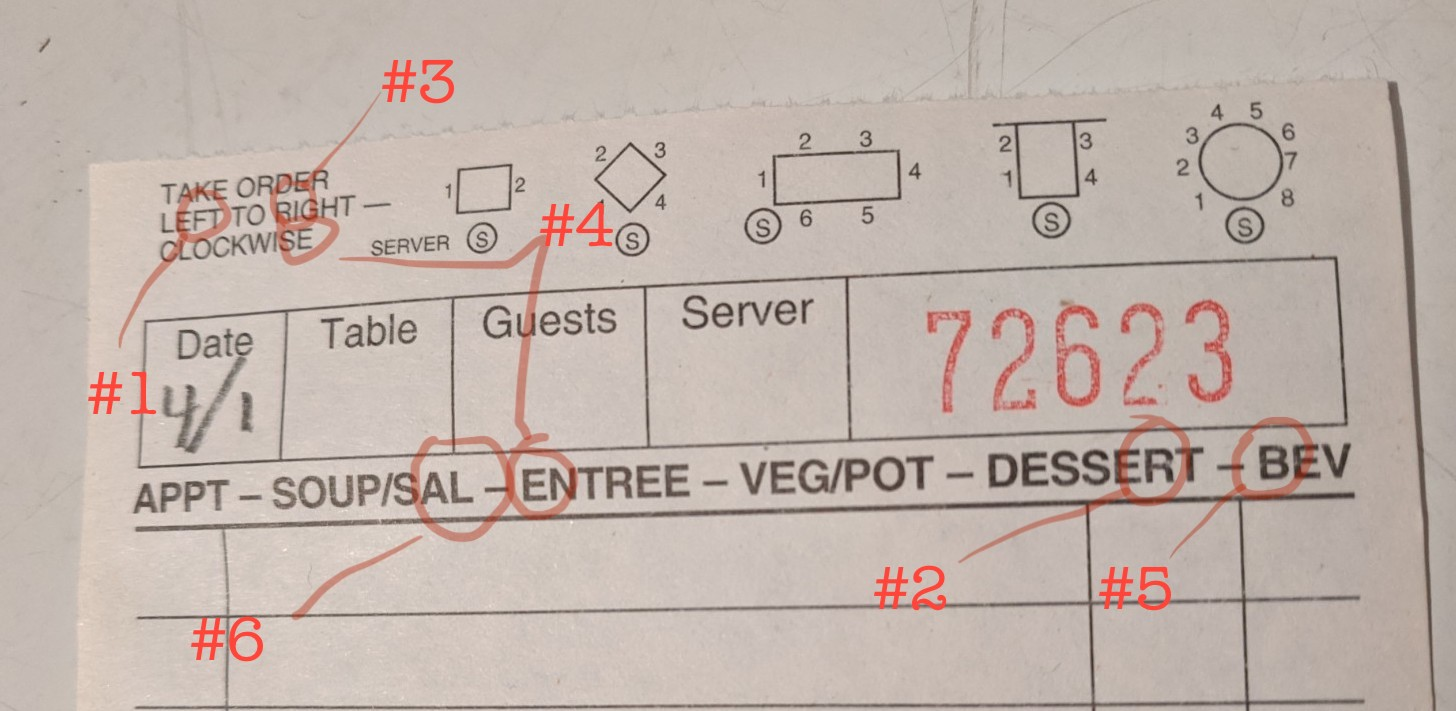
\includegraphics{cal-f1.jpg}[width=7in]
\end{figure}

\section*{Colophon}

Repo URL: \small\url{https://github.com/srl295/srl-unicode-proposals} 
Typeset by \LaTeX . Made with \( 100\%  \) recycled bits.

My GPG fingerprint is {\tt BA90 283A 60D6 7BA0 DD91  0A89 3932 080F 4FB4 19E3}
\end{document}
